\documentclass[10pt]{beamer}
%\documentclass[handout,dvips,11pt,grey]{beamer}
\usetheme{Goettingen}

%\usepackage{tikz,pgf}
\usepackage{multicol}
\usepackage{amsmath,amsthm,amssymb}
%\usepackage{epstopdf}
%\usepackage{xspace}
\usepackage{verbatim}
%\usepackage{circuitikz}
%\usepackage{graphicx}
%\usepackage{comment}
%\usepackage{array}
\usepackage{coffee4}

\title{Relevance Vector Machine}
\subtitle{Bayesian Extensions to Linear Systems}
\author{Philip Robinson}
\date{\today}
\institute{Presented to \\ OHSU - Machine Learning Class}

\begin{document}

\begin{frame}
  \titlepage
  \cofeAm{0.4}{0.5}{0}{3.5cm}{-2cm}
  \cofeCm{0.5}{0.5}{180}{0}{3cm}
\end{frame}


\begin{frame}{Presentation Overview}
  \cofeAm{0.3}{0.5}{0}{3.5cm}{-2cm}
  \cofeCm{0.4}{0.5}{180}{0}{3cm}

  \begin{itemize}
  \item Introduce SVM
  \item Introduce RVM
  \item Bayesianization
  \item Optimization Algorithm
  \item Existing Implementations
  \item Benchmarks
  \item Notes
  \end{itemize}
\end{frame}

\begin{frame}{Support Vector Machines}
  \cofeAm{0.2}{0.5}{0}{3.5cm}{-2cm}
  \cofeCm{0.3}{0.5}{180}{0}{3cm}

  \begin{multicols}{2}
    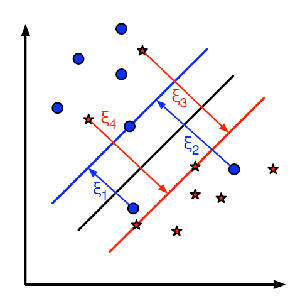
\includegraphics[width=\columnwidth]{./svm_basics3.png}
    \columnbreak

    SVMs hope to identify a decision boundary protected by the
    greatest margin. Ideally information is linearly separable, however
    in most cases you must fit a cost parameter. This is usually done
    with guesses or cross validation. {\em (expensive)}
  \end{multicols}

  \begin{itemize}
  \item non-informative classification
  \item only global minimum {\em (even over kernels)}
  \item only Mercer Kernels {\em ... idk}
  \end{itemize}

\end{frame}

\begin{frame}{Relevance Vector Machines}
  \cofeAm{0.1}{0.5}{0}{3.5cm}{-2cm}
  \cofeCm{0.2}{0.5}{180}{0}{3cm}

  \begin{quote}
    RVMs extend SVMs by adding Bayesian priors and weights \(\in \mathbb{R}^+\) to
    `support vectors` making `relevance vectors`.
  \end{quote}

  \begin{itemize}
  \item Gaussian priors to weights in training \;$\rightarrow$ regression
  \item Use of logistic sigmoid over regression $\rightarrow$ classification
  \item Informative classifications
  \item Preserves global minimum {\em (even over kernels)}
  \item Non-Mercer Kernels {\em ... idk}
  \item {\bf No closed form steps...}
  \end{itemize}

  \begin{quote}
    Priors on vector weights remove the need for cost parameters
  \end{quote}
\end{frame}

\begin{frame}{Bayesianization}
  \cofeAm{0.05}{0.5}{0}{3.5cm}{-2cm}
  \cofeCm{0.1}{0.5}{180}{0}{3cm}

  \begin{align*}
    \Phi &= \texttt{user kernel of machine} \\
    \phi_i(\vec{x}) &= \left[1, K(x, x_1), \ldots, K(x, x_N)\right]^T \\
    p(\vec{w}\;| \vec{\alpha}) &= \prod_{i=1}^N \mathcal{N}(w_i| 0, \alpha_i^{-1}) \\
    p(\vec{t}\;|\vec{w}, \sigma^2) &= (2\sigma^2)^{-\frac{N}{2}} exp\left\{- \frac{1}{2\sigma^2}\|\vec{t} - \Phi\vec{w}\|^2 \right\}\\
    p(\vec{w}\;|\vec{t}, \vec{\alpha}, \sigma^2) &= \frac{p(\vec{t}\;|\vec{w}, \sigma^2)p(\vec{w}|\;\vec{\alpha})}{p(\vec{t}\;|\vec{\alpha}, \sigma^2)} \\
    y(\vec{x}; \vec{w}) &= \sum_{i=1}^N w_i \phi_i(\vec{x}) \\
  \end{align*}

\end{frame}

\begin{frame}{Optimization Algorithm}

  \begin{itemize}
  \item Loop - Iterative Reweighted Least Squares, until $\vec{\alpha}$ converges
    \begin{itemize}
    \item \(\mbox{argmin}_{\vec{\mu}} \mathcal{L}(\vec{\mu}; \vec{\alpha}, \Phi, \vec{t})\)
      - Newton's Method, until $\vec{mu}$ converges
      \[\vec{\mu}_{i+1} = \vec{\mu}_i - (\nabla\nabla\mathcal{L}_{(\vec{\mu}_i)})^{-1} * \nabla\mathcal{L}_{(\vec{\mu}_i)}\]
    \item Iterative Re-estimation
      \begin{align*}
        \gamma_i &\equiv 1 - \alpha_i \Sigma_{ii}\\
        \alpha_i^{\texttt{new}} &= \frac{\gamma_i}{\mu_i^2}
      \end{align*}
    \item Prune large $\alpha_i$ and corresponding vectors from problem space
\end{itemize}
  \end{itemize}
\end{frame}

\begin{frame}{Existing Implementations}
  \begin{itemize}
  \item All use \texttt{BLAS} and \texttt{LAPACK}
  \item Python - uses \texttt{conjugate gradient}
  \item Matlab / C++ - Authors implementation
  \item R
  \end{itemize}
\end{frame}

\begin{frame}{UCI \texttt{wilt} dataset}
  \begin{itemize}
  \item identify sick trees from image summary statistics
  \item remote sensing problem
  \item labeled data, pre-split into test and train
  \end{itemize}
\end{frame}

\begin{frame}{Benchmarks}
  \begin{quote}
    to be included in report
  \end{quote}
\end{frame}

\begin{frame}{Next Steps}
  \begin{itemize}
  \item Extend to completely support regression
  \item Optimizations
    \begin{itemize}
    \item Incorporate \texttt{JuliaOpt} libraries for deeper \texttt{julia} integration
    \item Use \texttt{conjugate gradient}, or other faster strategy
    \end{itemize}
  \item Develop into \texttt{MLBase} conform-ant \texttt{julia} module
  \end{itemize}
\end{frame}

\begin{frame}{Notes}
  \begin{itemize}
  \item Check language and library defaults
  \item Don't disregard source material
  \item Use your type system
  \item Test with toy plus two `real' datasets
  \end{itemize}
\end{frame}

\end{document}
